\documentclass[preprint,12pt]{elsarticle}

\usepackage{caption}
\usepackage{hyperref}
\usepackage{graphicx}
\usepackage{subcaption}
\usepackage{amssymb}
\usepackage{amsmath}
\usepackage{multirow}
\usepackage[utf8]{inputenc}
\usepackage{cleveref}

% For the TODOs
\usepackage{xcolor}
\usepackage{xargs}
\usepackage[colorinlistoftodos,textsize=footnotesize]{todonotes}
\newcommand{\todoin}{\todo[inline]}
% from here: https://tex.stackexchange.com/questions/9796/how-to-add-todo-notes
\newcommandx{\unsure}[2][1=]{\todo[linecolor=red,backgroundcolor=red!25,bordercolor=red,#1]{#2}}
\newcommandx{\change}[2][1=]{\todo[linecolor=blue,backgroundcolor=blue!25,bordercolor=blue,#1]{#2}}
\newcommandx{\info}[2][1=]{\todo[linecolor=OliveGreen,backgroundcolor=OliveGreen!25,bordercolor=OliveGreen,#1]{#2}}

%Boldtype for greek symbols
\newcommand{\teng}[1]{\ensuremath{\boldsymbol{#1}}}
\newcommand{\ten}[1]{\ensuremath{\mathbf{#1}}}

\usepackage{lineno}

\journal{}

\begin{document}

\begin{frontmatter}

  \title{Rigid fluid coupling}
  \author[IITB]{Adepu Dinesh \corref{cor1}}
  \ead{adepu.dinesh.a@gmail.com} \author[IITB]{Prabhu Ramachandran}
  \ead{prabhu@aero.iitb.ac.in} \address[IITB]{Department of Aerospace
    Engineering, Indian Institute of Technology Bombay, Powai, Mumbai 400076}

\cortext[cor1]{Corresponding author}

\begin{abstract}
\end{abstract}

\begin{keyword}
%% keywords here, in the form: keyword \sep keyword
{XXX}, {XXX}, {XXX}

%% MSC codes here, in the form: \MSC code \sep code
%% or \MSC[2008] code \sep code (2000 is the default)

\end{keyword}

\end{frontmatter}

% \linenumbers

\section{Introduction}
\label{sec:intro}



\section{Governing equations}
\label{sec:fluid-mechanics}


\section{CTVF formulation}
\label{sec:ctvf-equations}


\section{SPH discretization}
\label{sec:sph-fluid-equations}


\section{Rigid body dynamics}
\label{sec:rbd}


\section{How to handle rigid fluid coupling}
\label{sec:rfc}


\section{Collision between rigid bodies}
\label{sec:contact-force}

\citet{chen2019coupled} has damping model. Also he mentioned the parameters
required in stack of cylinders example.


% \todoin{
% \begin{itemize}
% \item \citet{albano2016modelling} models using pure elastic impingement force
% % Development of the Resolved Fluid-Solid SPH Coupling using Rigid Body Dynamics
% \item \citet{choidevelopment} models using DEM
% \item \citet{zhan2020sph} uses hybrid contact model
% \end{itemize}
% A SPH framework for dynamic interaction between soil and rigid body system
% with hybrid contact method}



\section{Results and discussion}
\label{sec:results}

\subsection{3D Bouncing cube on a wall under gravity}
\label{sec:bouncing-cube}

In the current section we test the frictional part of the current solver by
modeling the sliding of a rigid body on an inclined surface in 3D. We compare
against the analytical solution to validate the test case.

We consider a rigid body of length 0.1 m, height 0.1 and depth of 0.1m allowed
to slide on an inclined surface at an angle $\frac{\pi}{3}$. A density of 2000
kg\,m\textsuperscript{-3} is used for the body. Other numerical parameters,
such as the repulsive spring stiffness $k_r=3.0 \times 10^{5}$ and tangential
spring stiffness $k_t=3.0 \times 10^{5}$ is chosen, respectively. A particle
spacing of $0.001$ is considered, resulting in $4400$ particles per body. From
the analytical solution, the evolution of velocity is given by,
\begin{equation}
  \label{eq:ce}
  \ten{v}(t) = (\mu \teng{g} \sin (\theta) - \teng{g} \cos (\theta)) t.
\end{equation}


We consider three different friction coefficients, $\mu=0.5$, $\mu=0.5$, and
$\mu=0.5$. From the analytical solution, when the friction coefficient is
greater than $\tan(frac{\pi}{3})$, the body doesn't slide.

\Cref{fig:dinesh-2022-bouncing-cube-snapshots-3d} depicts the snapshots of the
rigid body bouncing on a wall. The coefficient of restitution corresponding to
the snapshots are equal to $1$. As the rigid body approaches the wall, its
velocity is increases due to gravity. As soon as the body comes into contact
of the wall, the collision happens, the body's velocity is reduced until it
becomes zero, and then it rebounds, and bounces back to a certain height.



\begin{figure}[!htpb]
  \centering
  \begin{subfigure}{0.48\textwidth}
    \centering
    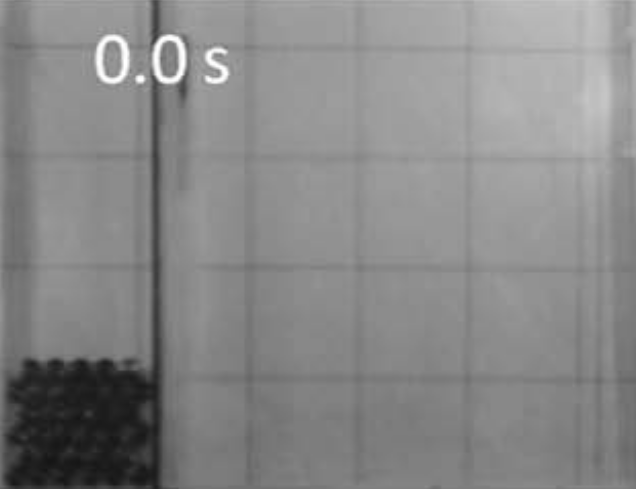
\includegraphics[width=1.0\textwidth]{figures/mohseni_2021_free_sliding_on_a_slope_3d/fric_coeff_0_4/time0}
    \subcaption{t = 2.5e-03 sec}\label{fig:passing-0}
  \end{subfigure}
  %
  \begin{subfigure}{0.48\textwidth}
    \centering
    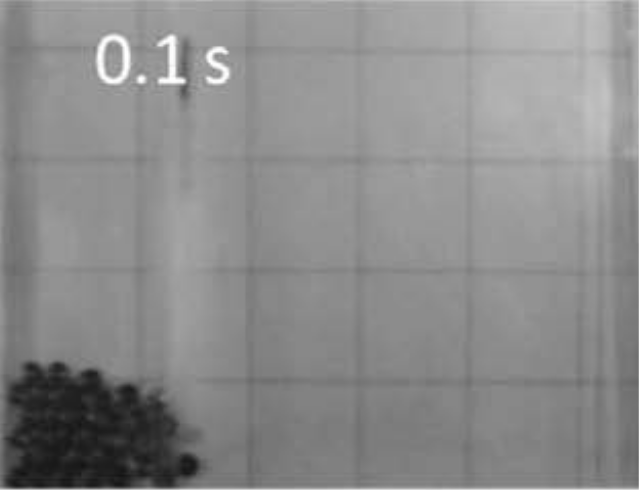
\includegraphics[width=1.0\textwidth]{figures/mohseni_2021_free_sliding_on_a_slope_3d/fric_coeff_0_4/time1}
    \subcaption{t = 2.5e-03 sec}\label{fig:passing-1}
  \end{subfigure}

  \begin{subfigure}{0.48\textwidth}
    \centering
    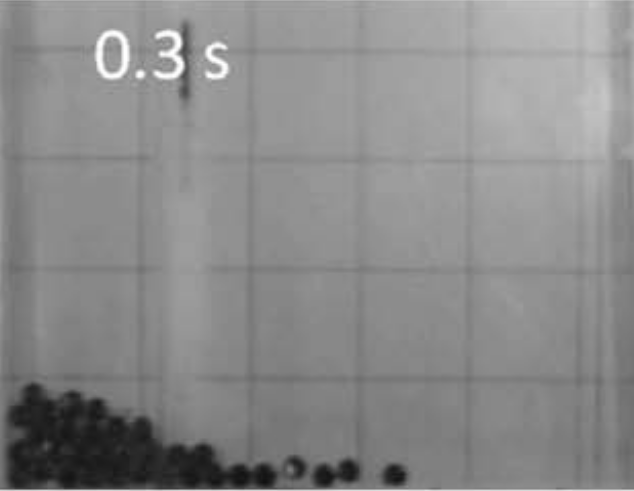
\includegraphics[width=1.0\textwidth]{figures/mohseni_2021_free_sliding_on_a_slope_3d/fric_coeff_0_4/time2}
    \subcaption{t = 2.5e-03 sec}\label{fig:passing-2}
  \end{subfigure}
  %
  \begin{subfigure}{0.48\textwidth}
    \centering
    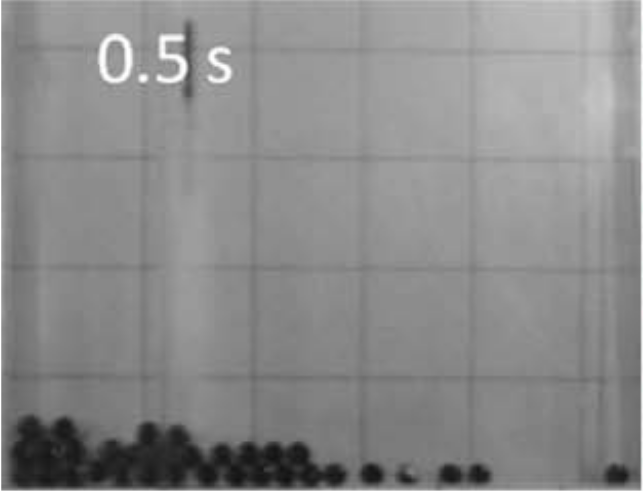
\includegraphics[width=1.0\textwidth]{figures/mohseni_2021_free_sliding_on_a_slope_3d/fric_coeff_0_4/time3}
    \subcaption{t = 2.5e-03 sec}\label{fig:passing-3}
  \end{subfigure}
  \caption{Elastic solid sliding}
\label{fig:mohseni-2021-sliding-3d}
\end{figure}
%

\Cref{fig:results-solid-sliding-velocity-vs-time} shows a evolution of
velocity of the center of mass of the rigid body for different frictional
coefficients against the analytical solution. From
\Cref{fig:results-solid-sliding-velocity-vs-time} we can see that the current
solver has an excellent match with the analytical solution and covers all the
regimes of the sliding case.


\begin{figure}[!htpb]
  \centering
  \includegraphics[width=0.4\textwidth]{figures/mohseni_2021_free_sliding_on_a_slope_3d/velocity_vs_time}
  \caption{Velocity versus time}
\label{fig:results-solid-sliding-velocity-vs-time}
\end{figure}


\subsubsection{A test to check the conservation properties of rigid body}
\label{sec:conservation-of-rb-properties}



\subsection{A 2d and 3d rigid body sliding}
\label{sec:rigid-body-sliding}

In the current section we test the frictional part of the current solver by
modeling the sliding of a rigid body on an inclined surface in 3D. We compare
against the analytical solution to validate the test case.

We consider a rigid body of length 0.1 m, height 0.1 and depth of 0.1m allowed
to slide on an inclined surface at an angle $\frac{\pi}{3}$. A density of 2000
kg\,m\textsuperscript{-3} is used for the body. Other numerical parameters,
such as the repulsive spring stiffness $k_r=3.0 \times 10^{5}$ and tangential
spring stiffness $k_t=3.0 \times 10^{5}$ is chosen, respectively. A particle
spacing of $0.001$ is considered, resulting in $4400$ particles per body. From
the analytical solution, the evolution of velocity is given by,
\begin{equation}
  \label{eq:ce}
  \ten{v}(t) = (\mu \teng{g} \sin (\theta) - \teng{g} \cos (\theta)) t.
\end{equation}


We consider three different friction coefficients, $\mu=0.5$, $\mu=0.5$, and
$\mu=0.5$. From the analytical solution, when the friction coefficient is
greater than $\tan(frac{\pi}{3})$, the body doesn't slide.

\Cref{fig:mohseni-2021-sliding-3d} shows the snapshots of the rigid body at 4
time instants. From \cref{fig:mohseni-2021-sliding-3d} we can see that the the
body is freely sliding with out having any oscillations or unphysical jumping
off the inclined wall. This is because of the new surface aware contact model
as force is not computed by considering the wall as spherical particles but by
ensemble of an overlap. The snapshots correspond to a friction coefficient of $0.4$.


\begin{figure}[!htpb]
  \centering
  \begin{subfigure}{0.48\textwidth}
    \centering
    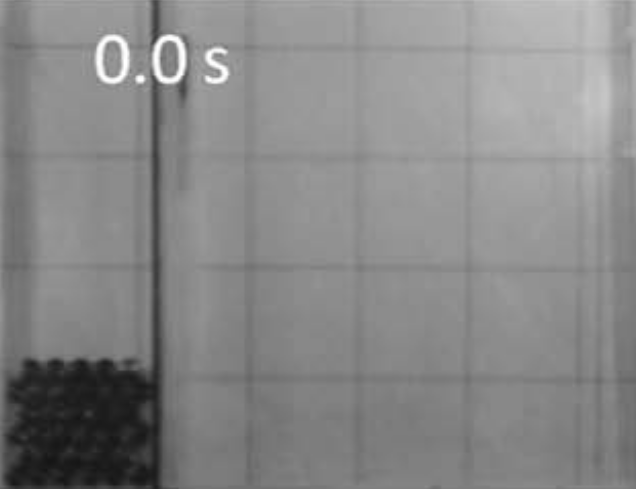
\includegraphics[width=1.0\textwidth]{figures/mohseni_2021_free_sliding_on_a_slope_3d/fric_coeff_0_4/time0}
    \subcaption{t = 2.5e-03 sec}\label{fig:passing-0}
  \end{subfigure}
  %
  \begin{subfigure}{0.48\textwidth}
    \centering
    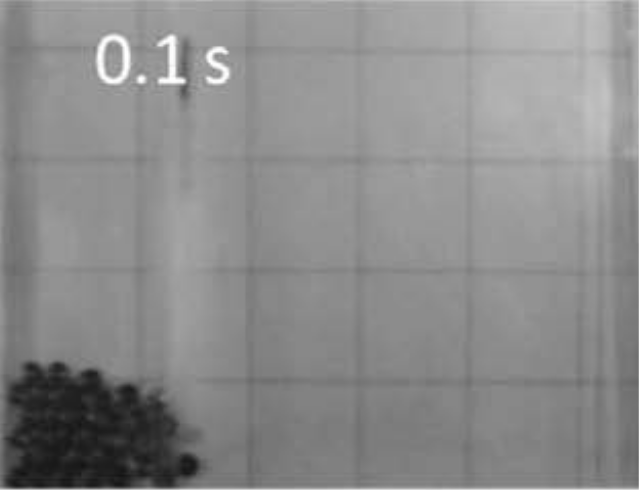
\includegraphics[width=1.0\textwidth]{figures/mohseni_2021_free_sliding_on_a_slope_3d/fric_coeff_0_4/time1}
    \subcaption{t = 2.5e-03 sec}\label{fig:passing-1}
  \end{subfigure}

  \begin{subfigure}{0.48\textwidth}
    \centering
    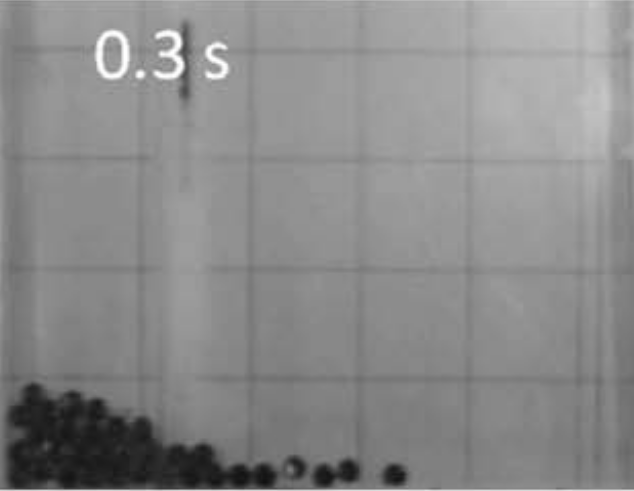
\includegraphics[width=1.0\textwidth]{figures/mohseni_2021_free_sliding_on_a_slope_3d/fric_coeff_0_4/time2}
    \subcaption{t = 2.5e-03 sec}\label{fig:passing-2}
  \end{subfigure}
  %
  \begin{subfigure}{0.48\textwidth}
    \centering
    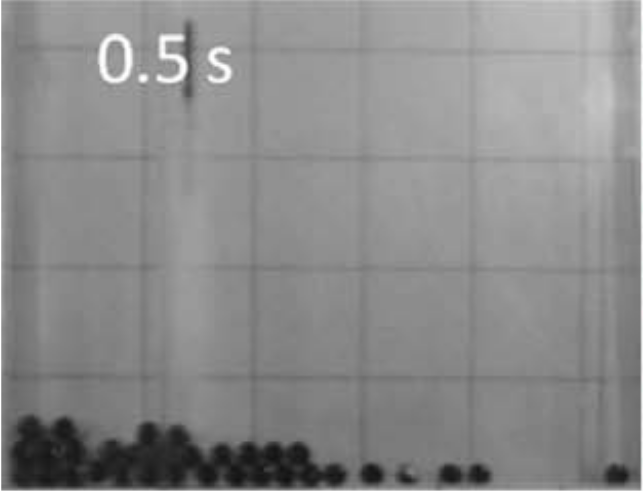
\includegraphics[width=1.0\textwidth]{figures/mohseni_2021_free_sliding_on_a_slope_3d/fric_coeff_0_4/time3}
    \subcaption{t = 2.5e-03 sec}\label{fig:passing-3}
  \end{subfigure}
  \caption{Elastic solid sliding}
\label{fig:mohseni-2021-sliding-3d}
\end{figure}
%

\Cref{fig:results-solid-sliding-velocity-vs-time} shows a evolution of
velocity of the center of mass of the rigid body for different frictional
coefficients against the analytical solution. From
\Cref{fig:results-solid-sliding-velocity-vs-time} we can see that the current
solver has an excellent match with the analytical solution and covers all the
regimes of the sliding case.


\begin{figure}[!htpb]
  \centering
  \includegraphics[width=0.4\textwidth]{figures/mohseni_2021_free_sliding_on_a_slope_3d/velocity_vs_time}
  \caption{Velocity versus time}
\label{fig:results-solid-sliding-velocity-vs-time}
\end{figure}


\subsection{Controlled Sliding on a Flat Surface}
\label{sec:controlled-rigid-body-sliding}



\subsection{Stack of cylinders}
\label{sec:stack-of-cylinders}



\subsection{Falling solid in water}
\label{sec:falling-solid-in-water}


\subsection{Floating solid in water}
\label{sec:floating-solid-in-water}


\subsection{3D dam breaking flow hitting one cube}
\label{sec:3d-dam-breaking-one-cube-hit}

\cite{amaro2019improvement}

\subsection{3D dam breaking flow hitting three cube}
\label{sec:3d-dam-breaking-one-cube-hit}

\cite{amaro2019improvement}

\subsection{3D dam breaking flow hitting pyramid cubes configuration}
\label{sec:3d-dam-breaking-one-cube-hit}

\cite{amaro2019improvement}


% \subsection{Dam break with body transport}
% \label{sec:dam-break-with-body-transport}

% \citet{wang2019numerical}

% \subsection{Dam break with multiple bodies transport}
% \label{sec:dam-break-with-multiple-bodies-transport}
% \citet{wang2019numerical}


% \subsection{Cylinders in water collapsed under gravity}
% \label{sec:cylinders-collapse-in-water}
% \citet{chen2019coupled}


\section{Conclusions}
\label{sec:conclusions}

\section*{References}
\bibliographystyle{model6-num-names}
\bibliography{references}



\end{document}

%%% Local Variables:
%%% mode: latex
%%% TeX-master: "paper"
%%% fill-column: 78
%%% End:
